\section{Grup Bebas}\label{sec:free-group}
Misalkan $X$ sebuah himpunan. Secara kasar, pada himpunan $X$, grup bebas $\mathbf{F}(X)$ adalah grup yang terdiri atas ungkapan-ungkapan yang dapat diperoleh dengan memulai dari unsur-unsur $X$, lalu melakukan perkalian dan pengambilan invers secara ``formal''. Ungkapan-ungkapan ini disebut \emph{kata} dalam grup bebas, dan $X$ disebut alfabetnya. Sebagai contoh, ketika $X=\{x,y\}$, $\mathbf{F}(X)$ adalah himpunan yang terdiri atas tak hingga banyak kata
\[ 1, x, y, x^{-1}, y^{-1}, xy, yx, x^2, yxy, \cdots \]
dan seterusnya. Kata ``bebas'' berarti bahwa perkalian kata tidak tunduk pada kendala apa pun selain syarat-syarat dasar teori grup, seperti hukum asosiatif dan $x x^{-1}=1$. Grup bebas dapat dicirikan oleh suatu sifat universal (lihat \S\ref{sec:cat-universals}). Kita juga akan membahas monoid bebas.

\begin{definition}[Monoid bebas]\label{def:free-monoid}\index{yaobanqun!monoid bebas (free monoid)}
	Perhatikan data berbentuk $(\mathbf{M}(X), \iota)$, dengan $\mathbf{M}(X)$ sebuah monoid dan $\iota: X \to \mathbf{M}(X)$ sebuah pemetaan himpunan. Jika untuk setiap monoid $M'$ dan pemetaan $\iota': X \to M'$, terdapat homomorfisme unik $\varphi: \mathbf{M}(X) \to M'$ yang membuat diagram berikut komutatif,
	\[ \begin{tikzcd}
		X \arrow[r, "\iota"] \arrow[rd, "{\iota'}"'] & \mathbf{M}(X) \arrow[dashed, d, "{\exists! \varphi}"] \\
		& M'
	\end{tikzcd} \]
	maka $(\mathbf{M}(X), \iota)$ disebut monoid bebas pada $X$.
\end{definition}

\begin{definition}[Grup bebas]\label{def:free-group}\index{qun!grup bebas (free group)}
	Perhatikan data berbentuk $(\mathbf{F}(X), \iota)$, dengan $\mathbf{F}(X)$ sebuah grup dan $\iota: X \to \mathbf{F}(X)$ sebuah pemetaan himpunan. Jika untuk setiap grup $G$ dan pemetaan $\iota': X \to G$, terdapat homomorfisme unik $\varphi: \mathbf{F}(X) \to G$ yang membuat diagram berikut komutatif,
	\[ \begin{tikzcd}
		X \arrow[r, "\iota"] \arrow[rd, "{\iota'}"'] & \mathbf{F}(X) \arrow[dashed, d, "{\exists! \varphi}"] \\
		& G
	\end{tikzcd} \]
	maka $(\mathbf{F}(X), \iota)$ disebut \emph{grup bebas} pada $X$.
\end{definition}

Dari definisi tersebut segera diperoleh beberapa sifat formal $\mathbf{M}(X)$ dan $\mathbf{F}(X)$. Sebagai contoh, setiap pemetaan $f: X \to Y$ menghasilkan sebuah diagram komutatif unik
\[ \begin{tikzcd}
	X \arrow[d, "f"'] \arrow[r, "{\iota_X}"] & \mathbf{M}(X) \arrow[d, "{\varphi_f}"] \\
	Y \arrow[r, "{\iota_Y}"'] & \mathbf{M}(Y)
\end{tikzcd} \]
dengan $\varphi_f$ sebuah homomorfisme: dalam sifat universal $\mathbf{M}(X)$, cukup ambil $M' = \mathbf{M}(Y)$ dan $\iota' = \iota_Y \circ f$. Jelas bahwa $\varphi_{\identity_X} = \identity_{\mathbf{M}(X)}$, sehingga $X \mapsto \mathbf{M}(X)$ menjadi sebuah fungtor. Demikian pula, $X \mapsto \mathbf{F}(X)$ memiliki sifat fungtorial serupa. Notasi $\iota$ sering dihilangkan.

\begin{remark}
	Dari sudut pandang lain, konstruksi grup bebas $X \mapsto (\mathbf{F}(X), \iota: X \to \mathbf{F}(X))$ menentukan fungtor adjoin kiri bagi fungtor pelupa $U: \cate{Grp} \to \cate{Set}$:
	\begin{align*}
		\Hom_\cate{Set}(X, G) & \longrightiso \Hom_\cate{Grp}(\mathbf{F}(X), G) \\
		\iota' & \longmapsto \varphi.
	\end{align*}
	Secara umum, salah satu prinsip dasar dalam aljabar adalah
	\begin{center}
		konstruksi bebas = fungtor adjoin kiri dari fungtor pelupa.
	\end{center}
	Kita akan menjumpai prinsip ini berulang kali ketika membahas konstruksi seperti gelanggang polinomial dan modul bebas.
\end{remark}
Untuk $X$ tertentu, pembahasan dalam \S\ref{sec:cat-universals} menunjukkan bahwa jika monoid bebas atau grup bebas ada, maka objek itu unik hingga isomorfisme unik. Sebagai contoh, andaikan data $(F_1, \iota_1)$ dan $(F_2, \iota_2)$ keduanya merupakan monoid bebas. Definisi memberikan homomorfisme-homomorfisme unik $\begin{tikzcd}[column sep=small] F_1 \arrow[r, yshift=0.5ex, "\varphi"] & F_2 \arrow[l, yshift=-0.5ex, "\psi"] \end{tikzcd}$ sedemikian sehingga $\varphi \iota_1 =\iota_2$ dan $\psi \iota_2 = \iota_1$. Dari keunikan diperoleh $ \varphi\psi \iota_2 = \iota_2 \implies \varphi\psi = \identity_{F_2}$, dan demikian pula $\psi\varphi = \identity_{F_1}$, sehingga keduanya merupakan isomorfisme yang dicari.

Semua yang diperlukan telah tersedia; tinggal memberikan konstruksinya. Kita mulai dengan monoid bebas $(\mathbf{M}(X), \iota)$. Definisikan $\mathbf{M}(X)$ sebagai himpunan ``kata'' berbentuk
\[ g := x_1 x_2  \cdots x_n, \qquad n \in \Z_{\geq 0}, \quad x_1, \ldots, x_n \in X \]
Secara ketat, kata $g$ adalah suatu barisan dalam $X$ dengan $n$ suku, yaitu $(x_i)_{i=1}^n$; $n$ disebut \emph{panjang} kata $g$. Ketika $n=0$, kata yang bersesuaian adalah kata kosong (yakni barisan kosong), yang dinotasikan dengan $1$.

Misalkan $g = x_1 \cdots x_n$ dan $h = y_1 \cdots y_m$ dua kata. Produk $gh$ tidak lain adalah konkatenasi kedua kata,
\[ gh := x_1 \cdots x_n y_1 \cdots y_m; \]
dari definisi, berlaku secara langsung $g \cdot 1 = g = 1 \cdot g$ dan hukum asosiatif $g(hk) = (gh)k$. Dengan demikian, $\mathbf{M}(X)$ memperoleh struktur monoid. Pemetaan $\iota: X \to \mathbf{M}(X)$ membawa $x \in X$ ke kata $x \in \mathbf{M}(X)$ yang panjangnya satu.

\begin{lemma}
	Data $(\mathbf{M}(X), \iota)$ yang dikonstruksi di atas adalah monoid bebas pada $X$.
\end{lemma}
\begin{proof}
	Untuk setiap monoid $M'$ dan pemetaan $\iota': X \to M'$, menurut Definisi \ref{def:free-monoid}, pemetaan $\varphi$ harus memenuhi
	\[ \varphi: x_1 \cdots x_n \longmapsto \iota'(x_1) \cdots \iota'(x_n), \quad x_1, \ldots, x_n \in X \]
	sehingga $\varphi$ unik. Berdasarkan konstruksi $\mathbf{M}(X)$, rumus di atas juga memberikan suatu $\varphi$ yang terdefinisi dengan baik.
\end{proof}

Strategi berikut mengonstruksi grup bebas dengan menggunakan produk teramalgamasi monoid.
\begin{definition}[Produk teramalgamasi]\label{def:amalgamated-product}\index{rongheji@produk teramalgamasi (amalgamated product)}
	Misalkan $(M_i)_{i \in I}$ suatu keluarga monoid. Diberikan sebuah monoid $A$ dan suatu keluarga homomorfisme $(f_i: A \to M_i )_{i \in I}$. Data $(M, (\varphi_i)_{i \in I})$ yang memenuhi sifat universal berikut disebut produk teramalgamasi dari $(M_i, f_i)_{i \in I}$:
	\begin{compactitem}
		\item $M$ adalah sebuah monoid; $\forall i \in I$, $\varphi_i: M_i \to M$ adalah sebuah homomorfisme;
		\item homomorfisme komposit $h := \varphi_i f_i: A \to M$ tidak bergantung pada $i$;
		\item jika data $(M', (\varphi'_i)_{i \in I})$ juga memenuhi sifat-sifat di atas, maka terdapat homomorfisme unik $\varphi: M \to M'$ yang membuat diagram berikut komutatif.
		\[ \begin{tikzcd}
			M_i \arrow[r, "{\varphi_i}"] \arrow[rd, "{\varphi'_i}"'] & M \arrow[d, "{\exists! \varphi}"] \\
			& M'
		\end{tikzcd} \]
	\end{compactitem}
\end{definition}

Karena produk teramalgamasi didefinisikan melalui sifat universal, produk itu tentu memiliki sifat keunikan yang lazim; kita tidak akan mengulang perinciannya. Berikut salah satu konstruksinya. Ambil gabungan saling lepas dari $M_i$ beserta monoid bebas yang bersesuaian,
\[ S :=  \bigsqcup_{i \in I} M_i, \quad \iota: S \to \mathbf{M}(S). \]
Kita ingin, di dalam $\mathbf{M}(S)$, menanamkan perkalian setiap $M_i$ dan mengidentifikasi citra-citra $f_i$. Perhatikan relasi ekuivalensi pada monoid $(\mathbf{M}(S), \cdot)$ yang dibangkitkan oleh
\begin{gather*}
	\underbracket{xy}_{\text{di dalam $M_i$}} \sim \underbracket{x \cdot y}_{\text{di dalam $\mathbf{M}(S)$}}, \quad i \in I, \; x,y \in M_i, \\
	\underbracket{1_i}_{\text{unsur identitas $M_i$}} \sim \underbracket{1}_{\text{unsur identitas $\mathbf{M}(S)$}}, \quad i \in I, \\
	f_i(a) \sim f_j(a), \quad i,j \in I, \; a \in A,
\end{gather*}
bersama \eqref{eqn:quotient-condition}; notasikan relasi ekuivalensi yang dihasilkan dengan $\sim$. Berdasarkan pembahasan struktur hasil bagi dalam \S\ref{sec:homomorphism}, himpunan hasil bagi
\[ M := \mathbf{M}(S)/\sim. \]
memiliki struktur monoid natural. Definisikan homomorfisme komposit $\varphi_i: M_i \to \mathbf{M}(S) \to M$. Dari konstruksi, homomorfisme $\varphi_i f_i$ tidak bergantung pada $i$; notasikan homomorfisme ini dengan $h: A \to M$. Selain itu, setiap unsur $M$ selalu dapat ditulis sebagai produk unsur-unsur berbentuk $\varphi_i(x)$, dengan $i \in I$.

\begin{lemma}
	Data $(M, (\varphi_i)_{i \in I})$ yang dikonstruksi di atas adalah produk teramalgamasi dari $(M_i, f_i)_{i \in I}$.
\end{lemma}
\begin{proof}
	Untuk data dalam Definisi \ref{def:amalgamated-product} yang berbentuk $(M' ,(\varphi'_i)_{i \in I})$, kita memperoleh secara berturut-turut
	\begin{compactenum}[(i)]
		\item sebuah homomorfisme $\mathbf{M}(S) \to M' $ yang membawa setiap unsur $x \in M_i$ ke $\varphi'_i(x)$ (gunakan Definisi \ref{def:free-monoid});
		\item sebuah homomorfisme $\varphi: M = (\mathbf{M}(S) /  \sim) \to M'$ yang membuat diagram
		\[\begin{tikzcd}[row sep=small, column sep=small]
			\mathbf{M}(S) \arrow[r] \arrow[d] & M' \\
			M=\mathbf{M}(S)/\sim \arrow[ru, "\varphi"']
		\end{tikzcd}\] komutatif (gunakan definisi relasi ekuivalensi $\sim$).
	\end{compactenum}
	Jelas bahwa $\varphi$ membuat diagram dalam Definisi \ref{def:amalgamated-product} komutatif. Karena citra-citra $\varphi_i$ membangkitkan $M$, pilihan ini unik.
\end{proof}

Berdasarkan konstruksi di atas, unsur produk teramalgamasi $M$ selalu dapat ditulis sebagai produk berhingga berbentuk
\[ m = \varphi_{i_1}(m_1) \varphi_{i_2}(m_2) \cdots \varphi_{i_n}(m_n), \qquad m_j \in M_{i_j} \]
dan, jika tidak menimbulkan kerancuan, kita menuliskannya secara ringkas sebagai
\[ m = m_1 \cdots m_n \quad \in M. \]
Jika setiap $m_j \in M_{i_j}$ invertibel, maka $m_1 \cdots m_n \in M$ juga invertibel, sebab
\begin{gather}\label{eqn:word-inverse}
	(m_1 \cdots m_n)^{-1} = m_n^{-1} \cdots m_1^{-1}.
\end{gather}
Sekarang kita perkenalkan syarat
\begin{equation}\label{eqn:free-product-condition}\begin{gathered}
	\forall i \in I, \; \exists \text{ subhimpunan }\; 1 \in H_i \subset M_i \; \text{ sedemikian sehingga }\;
	\begin{tikzcd}[column sep=small, row sep=tiny]
		A \times H_i \arrow[r, "1:1"] & M_i \\
		(a, x_i) \arrow[mapsto, r] \arrow[phantom, u, sloped, "\in" description] & f_i(a) x_i. \arrow[phantom, u, sloped, "\in" description]
	\end{tikzcd}
\end{gathered}\end{equation}
Tuliskan suatu unsur $M$ dalam bentuk $m = m_1 \cdots m_n$, dengan $m_j \in M_{i_j}$ dan $i_1, \ldots, i_n \in I$. Setelah menggabungkan faktor-faktor, kita dapat mengasumsikan bahwa indeks-indeks $i_j$ yang bersebelahan selalu berbeda. Menurut \eqref{eqn:free-product-condition}, tulis $m_j = f_{i_j}(a_j) x_j$, dengan $a_j \in A$ dan $x_j \in H_{i_j}$. Di dalam ungkapan $m$, kita ingin memindahkan semua $a_j$ ke ujung kiri. Untuk itu, cukup perhatikan kasus $n=2$: di dalam $M_{i_1}$, kita dapat menulis $x_1 f_{i_1}(a_2) = f_{i_1}(a'_2) x'_1$; sifat produk teramalgamasi $M$ lalu memastikan bahwa $h(a_1) x_1 h(a_2) x_2 = h(a_1) h(a'_2) x'_1 x_2$. Ungkapan yang diperoleh melalui proses ini,
\[ m = h(a) x_1 \cdots x_n \]
disebut \emph{tereduksi}; bilangan $n$ disebut \emph{panjang} ungkapan tersebut. Ungkapan tereduksi dengan panjang nol tidak lain adalah ungkapan berbentuk $h(a)$, dengan $a \in A$.

\begin{lemma}
	Andaikan $A$ dalam produk teramalgamasi memenuhi syarat \eqref{eqn:free-product-condition}. Maka setiap unsur memiliki representasi tereduksi yang unik, dan dua unsur sama jika dan hanya jika representasi tereduksinya sama. Khususnya, setiap $\varphi_i: M_i \to M$ bersifat injektif.
\end{lemma}
Jika setiap $f_i$ adalah homomorfisme injektif antargrup, syarat lemma dipenuhi secara otomatis: perhatikan aksi perkalian kiri $A$ melalui $f_i$ pada $M_i$, lalu pilih satu wakil dari setiap orbit untuk memperoleh $H_i$.

\begin{proof}
	Gagasan berikut tidak sulit, tetapi penulisan yang sepenuhnya ketat akan cukup panjang, sehingga kita hanya memberikan garis besarnya. Pilih suatu keluarga subhimpunan $(H_i \subset M_i)_{i \in I}$ yang memenuhi \eqref{eqn:free-product-condition}. Definisikan $\Sigma$ sebagai himpunan barisan berbentuk
	\[ [a; x_1, \ldots, x_n], \quad a \in A, \; n \geq 0, \; x_j \in H_{i_j}, x_j \neq 1, \]
	dengan $i_1, \ldots, i_n \in I$, dan kita juga mensyaratkan bahwa indeks-indeks $i_j$ yang bersebelahan berbeda. Definisikan pemetaan
	\begin{align*}
		\Phi: \Sigma & \longrightarrow M \\
		[a; x_1, \ldots, x_n] & \longmapsto h(a)x_1 \cdots x_n.
	\end{align*}
	Pemetaan ini membawa $[1]$ (ambil $n=0$) ke $1$. Penurunan representasi tereduksi sebelumnya menyiratkan bahwa $\Phi$ surjektif; tinggal membuktikan bahwa $\Phi$ injektif.

	Melalui $\Phi$, pada $\Sigma$ kita akan menyimulasikan aksi perkalian kiri $M$. Pertama, tetapkan $i \in I$. Definisikan aksi monoid $\alpha_i: M_i \times \Sigma \to \Sigma$ sebagai berikut. Setiap $\xi \in M_i$ memiliki representasi unik $\xi = f_i(a'') x$, dengan $a'' \in A$ dan $x \in H_i$. Untuk $\sigma = [a; x_1, \ldots, x_n] \in \Sigma$, definisikan $(a', x') \in A \times H_i$ yang muncul dalam rumus berikut dengan cara yang sama seperti pada paragraf sebelumnya:
	\[ \alpha_i(\xi, \sigma) :=
	\begin{cases}
		[a'' a'; x', x_2, \ldots, x_n], \;\text{dengan}\; x f_i(a) x_1 = f_i(a') x', & i_1 = i, \\
		[a'' a'; x', x_1, \ldots, x_n], \;\text{dengan}\; x f_i(a) = f_i(a') x', & i_1 \neq i.
	\end{cases} \]
	Definisikan pula aksi $\alpha_A: A \times \Sigma \to \Sigma$ dengan $\alpha_A(a, [b; \ldots]) = [ab; \ldots]$. Pandang aksi-aksi ini sebagai keluarga homomorfisme $M_i \to \End(\Sigma)$ dan $A \to \End(\Sigma)$, dengan $\End(\Sigma)$ menyatakan monoid semua pemetaan $\Sigma \to \Sigma$.

	Berdasarkan sifat universal produk teramalgamasi, semua homomorfisme di atas dapat direkatkan menjadi $M \to \End(\Sigma)$, yakni sebuah aksi monoid $\alpha: M \times \Sigma \to \Sigma$. Mudah dibuktikan bahwa
	\[ \alpha(\Phi(\sigma), [1]) = \sigma, \quad \sigma \in \Sigma. \]
	Dengan demikian, segera diperoleh bahwa $\Phi$ injektif.
\end{proof}

\begin{proposition}
	Misalkan $X$ sebuah himpunan. Dalam Definisi \ref{def:amalgamated-product}, ambil $I = X$, $A = \{1\}$, dan untuk setiap $x \in X$ ambil $M_x := \Z$ (sebagai grup aditif); notasikan produk teramalgamasi tersebut dengan $(\mathbf{F}(X), (\iota_x)_{x \in X})$. Definisikan $\iota(x) = \iota_x(1)$. Maka $(\mathbf{F}(X), \iota)$ adalah grup bebas pada $X$.
\end{proposition}
\begin{proof}
	Menurut \eqref{eqn:word-inverse}, $\mathbf{F}(X)$ adalah sebuah grup. Untuk memverifikasi sifat universalnya, diberikan sebuah grup $G$ dan pemetaan $\iota': X \to G$, definisikan untuk setiap $x \in X$ homomorfisme
	\begin{align*}
		\varphi'_x: \Z & \longrightarrow G, \\
		a & \longmapsto \iota'(x)^a.
	\end{align*}
	Keluarga homomorfisme ini memenuhi syarat dalam Definisi \ref{def:amalgamated-product}, sehingga terdapat homomorfisme unik $\varphi: \mathbf{F}(X) \to G$ sedemikian sehingga
	\[ \varphi(\iota_x(a)) = \varphi'_x(a) = \iota'(x)^a, \quad x \in X, \; a \in \Z.  \]
	Berdasarkan sifat homomorfisme grup, rumus di atas dapat direduksi ke kasus $a=1$, yakni $\varphi(\iota(x)) = \iota'(x)$, yang tepat merupakan sifat universal grup bebas.
\end{proof}

Dari pembahasan produk teramalgamasi, unsur-unsur $\mathbf{F}(X)$ dapat ditulis dalam bentuk $\iota_x(a) \iota_y(b) \cdots$, dengan $x, y, \ldots \in X$ dan $a, b, \ldots \in \Z$; kita menuliskannya secara ringkas sebagai $x^a y^b \cdots$. Selanjutnya, setiap pangkat dapat diuraikan sehingga $a, b, \ldots \in \{\pm 1\}$. Ungkapan dalam $\mathbf{F}(X)$ yang berbentuk
\[ x_1^{\pm 1} \cdots x_n^{\pm 1}, \quad x_1, \ldots, x_n \in X,  \; (\text{ pengulangan diperbolehkan }) \]
disebut \emph{kata}. Sejalan dengan itu, kita dapat mendefinisikan konsep \emph{kata tereduksi}. Untuk $g \in \mathbf{F}(X)$, definisikan \emph{panjang}nya sebagai panjang minimum di antara semua ungkapan semacam itu. Jelas bahwa $\ell(g)=0 \iff g=1$, sedangkan $\ell(g)=1 \iff g \in \iota(X) \sqcup \iota(X)^{-1}$.

Produk teramalgamasi juga berguna di luar konstruksi ini. Perhatikan situasi berikut: dalam Definisi \ref{def:amalgamated-product}, andaikan $A$ dan setiap $M_i = G_i$ adalah grup, serta $f_i$ injektif. Produk teramalgamasi yang bersesuaian dinotasikan dengan $\ast_{\substack{i \in I \\ A}} G_i$. Menurut \eqref{eqn:word-inverse}, $\ast_{\substack{i \in I \\ A}} G_i$ adalah sebuah grup. Grup ini dilengkapi keluarga morfisme $\iota_i: G_i \to \ast_{\substack{i \in I \\ A}} G_i$.

\begin{definition}[Produk bebas]\label{def:free-product}\index{ziyouji@produk bebas (free product)}
	Misalkan $I$ sebuah himpunan dan $(G_i)_{i \in I}$ suatu keluarga grup. Ambil $A = \{1\}$ dalam definisi produk teramalgamasi. Data $(\ast_{i \in I} G_i, (\iota_i)_{i \in I})$ yang diperoleh disebut produk bebas dari $(G_i)_{i \in I}$. Jika $I$ adalah himpunan berhingga $\{1, \ldots, n\}$, kita juga menulisnya sebagai $G_1 \ast \cdots \ast G_n$.
\end{definition}
Sifat universalnya serupa dengan Definisi \ref{def:amalgamated-product}; perumusannya diserahkan kepada pembaca.

Selanjutnya, kita perhatikan kasus komutatif. Sekali lagi kita mulai dari sifat universal dan akan menyajikannya sesingkat mungkin. Semua operasi biner pada monoid komutatif berikut ditulis secara aditif.
\begin{definition}[Monoid komutatif bebas dan grup komutatif bebas]\label{def:free-comm-monoid}
	Misalkan $X$ sebuah himpunan. Jika data $(M, \iota)$ memenuhi
	\begin{inparaenum}[(i)]
		\item $M$ adalah monoid komutatif,
		\item $\iota: X \to M$ adalah sebuah pemetaan,
		\item untuk setiap data $(M', \iota')$ seperti di atas, terdapat homomorfisme unik $\varphi: M \to M'$ yang membuat diagram
			\begin{tikzcd}[row sep=small, column sep=small]
				X \arrow[r, "\iota"] \arrow[rd, "{\iota'}"'] & M \arrow[d, "\varphi"] \\
				& M'
			\end{tikzcd}
			komutatif.
	\end{inparaenum}
	maka $(M, \iota)$ disebut monoid komutatif bebas pada $X$. Jika dalam syarat-syarat tersebut $M, M'$ diwajibkan menjadi grup komutatif, kita memperoleh konsep grup komutatif bebas.
\end{definition}
Kita akan menggunakan jumlah langsung untuk konstruksinya.
\begin{proposition}\label{prop:monoid-direct-sum}
	Misalkan $(M_i)_{i \in I}$ suatu keluarga monoid komutatif. Definisikan \emph{jumlah langsung}nya sebagai submonoid
	\[ \begin{aligned} \bigoplus_{i \in I} M_i &:= \Bigl\{ (m_i)_{i \in I} \in \prod_{i \in I} M_i : {} \\ &\qquad \text{untuk semua kecuali paling banyak berhingga banyak $i$}, \; m_i = 0 \Bigr\}. \end{aligned} \]
	Berkenaan dengan morfisme inklusi $\iota_j: M_j \to \bigoplus_{i \in I} M_i$ (yakni penyisipan pada posisi ke-$j$), sifat universal berikut berlaku: untuk setiap keluarga homomorfisme monoid komutatif $\iota'_j: M_j \to M'$, diagram berikut komutatif.
	\[ \begin{tikzcd}
		M_j \arrow[r, "\iota_j"] \arrow[rd, "{\iota'_j}"'] & \bigoplus_{i \in I} M_i \arrow[d, "{\exists! \varphi}"] \\
		& M'
	\end{tikzcd} \]
\end{proposition}
\begin{proof}
	Satu-satunya pilihan yang mungkin adalah $\varphi: (m_i)_{i \in I} \mapsto \sum_{i \in I} \iota'_i(m_i)$, dan jumlah terakhir ini berhingga.
\end{proof}

Kembali ke monoid komutatif bebas pada $X$. Dengan himpunan indeks $X$, konstruksinya adalah jumlah langsung dari salinan-salinan $\Z_{\geq 0}$,
\[ \begin{aligned} \Z_{\geq 0}^{\oplus X} &:= \Bigl\{ \text{jumlah formal } \; \sum_{x \in X} a_x \cdot x : {} \\ &\qquad \forall x, \; a_x \in \Z_{\geq 0}, \; \text{hanya berhingga banyak suku yang tak nol} \Bigr\}. \end{aligned} \]
Istilah ``jumlah formal'' berarti bahwa $\sum_x a_x x$ sebenarnya harus dipandang sebagai keluarga unsur $(a_x)_{x \in X}$. Pemetaan $\iota: X \to \Z_{\geq 0}^{\oplus X}$ diberikan oleh $\iota(x) = 1 \cdot x =: x$.

Jika dalam definisi di atas monoid $\Z_{\geq 0}$ diganti dengan grup $\Z$, kita memperoleh grup komutatif bebas $(\Z^{\oplus X}, \iota)$. Perhatikan bahwa $-(\sum_x a_x x) = \sum_x (-a_x) x$.

\begin{proposition}
	Setiap grup $G$ dapat ditulis sebagai grup hasil bagi dari suatu grup bebas. Lebih tepatnya, jika subhimpunan $X \subset G$ membangkitkan $G$, maka inklusi $X \hookrightarrow G$ menginduksi homomorfisme surjektif $p: \mathbf{F}(X) \to G$.
\end{proposition}
\begin{proof}
	Homomorfisme $p$ membawa kata dalam $\mathbf{F}(X)$ yang berbentuk $x_1^{\pm 1} \cdots x_n^{\pm 1}$ ke $x_1^{\pm 1} \cdots x_n^{\pm 1} \in G$, sehingga $\Image(p) = \lrangle{X}$.
\end{proof}

Unsur-unsur subgrup normal $\Ker(p) \lhd \mathbf{F}(X)$ dapat dipandang sebagai \emph{relasi} yang dipenuhi oleh pembangkit-pembangkit $X$ di dalam $G$, dan kita ingin mendeskripsikannya dengan suatu himpunan pembangkit. Secara tepat, untuk setiap grup $\mathcal{G}$ dan subhimpunannya $Y$, definisikan $\lrangle{Y}_{\text{nor}}$ sebagai subgrup normal terkecil dalam $\mathcal{G}$ yang memuat $Y$. Sebagai subgrup, objek ini dibangkitkan oleh $\left\{ gyg^{-1}: y \in Y, \; g \in \mathcal{G} \right\}$. Kita ingin memilih $Y \subset \mathbf{F}(X)$ sedemikian sehingga $\lrangle{Y}_{\text{nor}} = \Ker(p)$; hal ini membawa kita pada konsep berikut.

\begin{definition}[Presentasi grup]\index{qunzhanshi@presentasi grup (group presentation)}
	Sebuah \emph{presentasi} grup $G$ terdiri atas suatu himpunan $X$, suatu subhimpunan $Y \subset \mathbf{F}(X)$, dan sebuah isomorfisme
	\[ \mathbf{F}(X)/\lrangle{Y}_{\mathrm{nor}} \rightiso G; \]
	Jika $X$ dapat dipilih berhingga, maka $G$ disebut \emph{dibangkitkan secara berhingga}; jika $X, Y$ keduanya dapat dipilih berhingga, maka $G$ disebut \emph{dipresentasikan secara berhingga}. \index{youxianshengcheng@dibangkitkan secara berhingga (finitely generated)} \index{youxianzhanshi@dipresentasikan secara berhingga (finitely presented)}
\end{definition}
Singkatnya, presentasi = pembangkit + relasi. Presentasi berhingga lazim ditulis dalam bentuk
\[ G = \lrangle{ \; x_1, \ldots, x_n  \big| w_1=1, \ldots, w_m=1 \; } \]
dengan $X = \{x_1, \ldots, x_n\}$ dan $\Ker[\mathbf{F}(X) \to G] = \lrangle{w_1, \ldots, w_m}_\text{nor}$.

\begin{example}\label{eg:dihedral-presentation}
	Untuk $n \in \Z_{\geq 1}$, grup dihedral $D_{2n}$ dari Contoh \ref{eg:dihedral-group} memiliki presentasi
	\[ D_{2n} = \lrangle{ a, b \big| a^n=1, b^2=1, b^{-1}ab = a^{-1}  }. \]
	Dengan notasi Contoh \ref{eg:dihedral-group}, pembangkit $a$ di dalam $\Z/n\Z$ bersesuaian dengan pembangkit $1+n\Z$, sedangkan $b$ bersesuaian dengan $\tau \in \Z/2\Z$. Kita juga dapat menggunakan pembangkit $\sigma := ab$ dan $\tau := b$ untuk memberikan presentasi lain,
	\[ D_{2n} \simeq \lrangle{ \sigma, \tau \big| \sigma^2=1, \tau^2 = 1, (\sigma\tau)^n=1}. \]
\end{example}

\begin{example}
	R.\ Guralnick dan G.\ Malle membuktikan bahwa setiap grup sederhana berhingga yang nonkomutatif dapat dibangkitkan oleh dua unsur yang saling konjugat; lihat \cite[Corollary 8.3]{GM12}. Tentu saja, relasi di antara keduanya dapat sangat rumit. Teknik pembuktiannya berliku dan bergantung pada klasifikasi grup sederhana berhingga serta teori representasi grup yang cukup mendalam.
\end{example}

Ingat bahwa tujuan awal kita adalah menyelidiki struktur $G$. Untuk suatu presentasi berhingga, M.\ Dehn \cite{De11} mengajukan masalah-masalah berikut.
\begin{description}
	\item[Masalah kata] Bagaimana menentukan apakah suatu kata $w \in \mathbf{F}(X)$ termasuk dalam $\lrangle{Y}_{\mathrm{nor}}$?
	\item[Masalah konjugasi] Bagaimana menentukan apakah citra dua kata $w, w' \in \mathbf{F}(X)$ saling konjugat di dalam $G$?
	\item[Masalah isomorfisme] Bagaimana menentukan apakah dua presentasi berhingga memberikan grup-grup yang isomorfik?
\end{description}
Ketiga masalah tersebut secara algoritmik tidak dapat diputuskan, tetapi algoritme tersedia untuk kelas-kelas grup tertentu (misalnya grup kepang $\mathcal{B}_n$). Masalah-masalah semacam ini termasuk dalam \emph{teori grup kombinatorial}, yang tidak akan dibahas secara terperinci dalam buku ini. Pembaca dapat memperoleh gambaran tentang kerumitannya dalam pembuktian Teorema \ref{prop:S_n-presentation}. Kajian tentang keterputusan (decidability), atau keterkomputasian (computability), merupakan salah satu cabang logika matematika yang disebut \emph{teori rekursi}.

\begin{theorem}[Nielsen--Schreier]
	Setiap subgrup dari grup bebas juga merupakan grup bebas.
\end{theorem}
\begin{proof}
	Kita menggunakan argumen topologis. Perhatikan grup bebas $\mathbf{F}(X)$; demi intuisi, pembaca boleh mengasumsikan bahwa $X$ berhingga selama argumen ini. Misalkan $(B_X, \star)$ adalah ruang topologis bertitik dasar yang diperoleh sebagai berikut: untuk setiap unsur dari $X$, ambil satu salinan $\mathbb{S}^1$, lalu rekatkan semua salinan tersebut pada satu titik. Sebagai contoh, ketika $|X|=4$:
	\[ B_X \; = \; 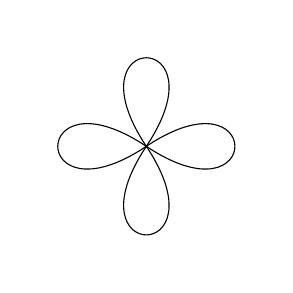
\begin{tikzpicture}[baseline=(current bounding box.center)]
		\draw (0,0) .. controls (1, 1.5) and (-1, 1.5) .. (0,0);
		\draw[rotate=90] (0,0) .. controls (1, 1.5) and (-1, 1.5) .. (0,0);
		\draw[rotate=180] (0,0) .. controls (1, 1.5) and (-1, 1.5) .. (0,0);
		\draw[rotate=270] (0,0) .. controls (1, 1.5) and (-1, 1.5) .. (0,0);
	\end{tikzpicture}\]
	Kita mengklaim adanya isomorfisme grup $\mathbf{F}(X) \rightiso \pi_1(B_X, \star)$ yang membawa $x \in X$ ke lintasan di $B_X$ yang berawal di $\star$ dan mengelilingi satu kali, dalam arah positif, salinan berlabel $x$ dari $\mathbb{S}^1$. Ketika $|X|=1$, ini tidak lain adalah isomorfisme yang lazim $\pi_1(\mathbb{S}^1, \star) \rightiso \Z$ \cite[Bab IV \S 3.1]{You}. Kasus umum mengikuti dari teorema van Kampen; versi berhingganya dapat ditemukan dalam \cite[Lampiran B]{You}.

	Ingat kembali konsep graf. Sebuah graf $\Gamma = (V, E, s, t)$ terdiri atas himpunan verteks $V$ dan himpunan sisi $E$; setiap sisi memiliki ujung awal dan ujung akhir yang ditentukan oleh sepasang pemetaan $s, t: E \to V$. Dari $\Gamma$ dapat dikonstruksi realisasi geometriknya $|\Gamma|$: secara konkret, ambil satu salinan interval $[0, 1]$ untuk setiap sisi, lalu rekatkan interval-interval tersebut pada verteks-verteks untuk membentuk $|\Gamma|$. Selanjutnya kita mengidentifikasi $\Gamma$ dengan $|\Gamma|$, sehingga graf yang dibahas dianggap tak berarah. Ruang $B_X$ yang didefinisikan sebelumnya adalah graf dengan satu verteks. Sebuah hasil dasar teori graf menyatakan bahwa jika $\Gamma$ terhubung, maka terdapat pohon rentang maksimal $T$: suatu subgraf dari $\Gamma$ yang memuat setiap verteks $\Gamma$ dan tidak memuat sirkuit. Secara intuitif, di dalam $\Gamma$ kita dapat mengontraksikan pohon $T$ secara kontinu ke suatu verteks $\star$ (ini disebut retraksi deformasi; lihat \cite[Bab IV \S 4.3]{You}). Sebagai contoh, dengan mengontraksikan pohon rentang maksimal yang ditandai garis tebal dalam gambar berikut, kita memperoleh kembali semanggi berdaun empat di atas.
	\begin{center}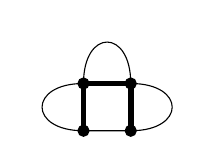
\begin{tikzpicture}[every node/.style={circle, draw, fill=black}, bentcurve/.style={bend left=90, looseness=3} ]
		\begin{scope}[scale=0.6]
			\coordinate (A) at (0,0) {};
			\coordinate (B) at (0,1) {};
			\coordinate (C) at (1,1) {};
			\coordinate (D) at (1, 0) {};
		\end{scope}
		\draw [line width=2pt] (A) -- (B) -- (C) -- (D);
		\draw[bentcurve] (A) to (B) to (C) to (D) --cycle;
		\foreach \x in {A, B, C, D}
			\draw[circle, fill=black] (\x) circle[radius=2pt];
	\end{tikzpicture}\end{center}
	Dalam kasus umum, karena $T$ memuat semua verteks, ruang hasil bagi $\Gamma/T$ akan homeomorfik dengan suatu $B_Y$. Oleh karena itu,
	\[ \pi_1(\Gamma, \star)  \rightiso \pi_1(\Gamma/T, \star) \simeq \pi_1(B_Y, \star) \; \text{adalah grup bebas}. \]
	Tetapkan suatu himpunan $X$. Teori ruang penutup \cite[Bab V \S 4]{You} menyatakan bahwa untuk $\mathbf{F}(X) \simeq \pi_1(B_X, \star)$ dan setiap subgrupnya $H$, terdapat ruang penutup $\widetilde{B_X} \to B_X$ sedemikian sehingga $H$ adalah citra homomorfisme injektif $\pi_1\left( \widetilde{B_X}, \star \right) \to \pi_1(B_X, \star)$. Dengan demikian, kita hanya perlu membuktikan bahwa $\pi_1\left(\widetilde{B_X}, \star\right)$ bebas; klaim ini tereduksi pada sifat berikut:
	\begin{center} Ruang penutup dari suatu graf tetap merupakan graf. \end{center}
	Ini adalah akibat langsung dari sifat pengangkatan lintasan untuk ruang penutup.
\end{proof}
